\documentclass[a4paper, 10pt]{article}
\usepackage{helvet}
\renewcommand{\familydefault}{\sfdefault}
\usepackage{pgf}
\usepackage{eurosym}
\usepackage{graphicx}
\usepackage{wasysym}
\usepackage{hyperref}
\usepackage{listings}
\usepackage{pxfonts}
\usepackage{verbatim}
\usepackage{color}
\usepackage{xcolor}
\usepackage{wrapfig}
\usepackage{enumitem}
\usepackage{booktabs}
\usepackage{gensymb}
\usepackage{tabularx}
\usepackage{currfile}

\hypersetup{
    bookmarks=true,         % show bookmarks bar?
    unicode=true,          % non-Latin characters in Acrobat’s bookmarks
    pdftoolbar=true,        % show Acrobat’s toolbar?
    pdfmenubar=true,        % show Acrobat’s menu?
    pdffitwindow=true,     % window fit to page when opened
    pdftitle={Assessments},    % title
    pdfauthor={Paul Vesey},     % author
    pdfsubject={Building Information Modelling },   % subject of the document
    pdfcreator={},   % creator of the document
    pdfproducer={xelatex}, % producer of the document
    pdfkeywords={'Graphics' }, % list of keywords
    pdfnewwindow=true,      % links in new PDF window
    colorlinks=true,       % false: boxed links; true: colored links
    linkcolor=violet,          % color of internal links (change box color with linkbordercolor)
    citecolor=magenta,        % color of links to bibliography
    filecolor=red,      % color of file links
    urlcolor=blue           % color of external links
}

\setlength\parindent{0pt}
\begin{document}

\lstset{language=HTML,
				basicstyle=\small,
				breaklines=true,
        numbers=left,
        numberstyle=\tiny,
        showstringspaces=false,
        aboveskip=-20pt,
        frame=leftline
        }


\begin{figure}
	\centering
	\includegraphics[width=0.5\linewidth]{./img/TUSlogo}
\end{figure}


\begin{tabularx}{\textwidth}{ |l|X| }
	\hline
	
	\textbf{Subject:} & Health \& Safety IT\\
	\textbf{Course:} & BSc in Construction Health \& Safety\\
	\textbf{Session:} & Autumn 2021\\
	\textbf{Lecturer:} & Paul Vesey \footnotesize{BEng, MIE, HDip}\\
	\textbf{Filename:} & \currfilebase\\
	\hline
\end{tabularx}

	
\part*{Assignment 1 (33\%) - Python with Excel}

\begin{tabularx}{\textwidth}{ |X|X| }
	\hline
	\textbf{Issue Date:} & 28$^{th}$ October 2021 \\
	\hline 
	\textbf{Submission Date:}  & 27$^{th}$ November 2021  \\
	\hline
\end{tabularx}


\section*{Continuous Assessment}
This assignment will account for 33\% of the 100\% allocated for continuous assessment in this module under COVID-19 regulations


\section*{Background Information}

Administrative tasks can consume considerable resources within organisations.  The documentation requirements within the health and safety domain leads often adds to this administrative overhead.  Automating aspects of administrative works increases efficiency, while at the same time providing opportunities to yield data insights not normally achievable.


\section*{Assignment Outline}

The Health and Safety Authority has produced a checklist document that employers can use to gather data from employees before they return to work.  A copy of this form is provided in pdf and Excel format within the asset pack of this assignment.  Given the likelihood that forms like this will be issued to numerous employees, and that they need to be tracked and controlled, it offers a good opportunity for automation.\\
\\
In this assignment you will automate the production of partially populated forms for each of the 12 employees listed below.\\

\begin{tabularx}{\textwidth}{ |X|X|X| }
	\hline
	Alice Adams & Bob Baker & Carol Clark \\
	Dan Davis & Erin Evans & Faythe Frank \\
	Grace Ghosh & Heidi Hills & Ivan Irwin \\
	John Jones & Kevin Klein & Lisa Lopez \\
	\hline
\end{tabularx}

\vspace{0.5cm}

For each of these employees, you are to create an excel version of the form customised with the name of the employee.  To do this, you are required to use batch files and the Python programming language with the \textit{OpenPyXL} package.\\

\section*{Approach}

The creation of the individual Excel files is to be carried out using a Windows batch (.bat) file.  Python can then be used to iterate over each of these files and insert the name of the employee in the correct cell of the file, along with their manager name and workplace address.  The fields to be populated with your programme are indicated in Figure \ref{fig:hsaform}\\

\begin{figure}[h]
	\centering
	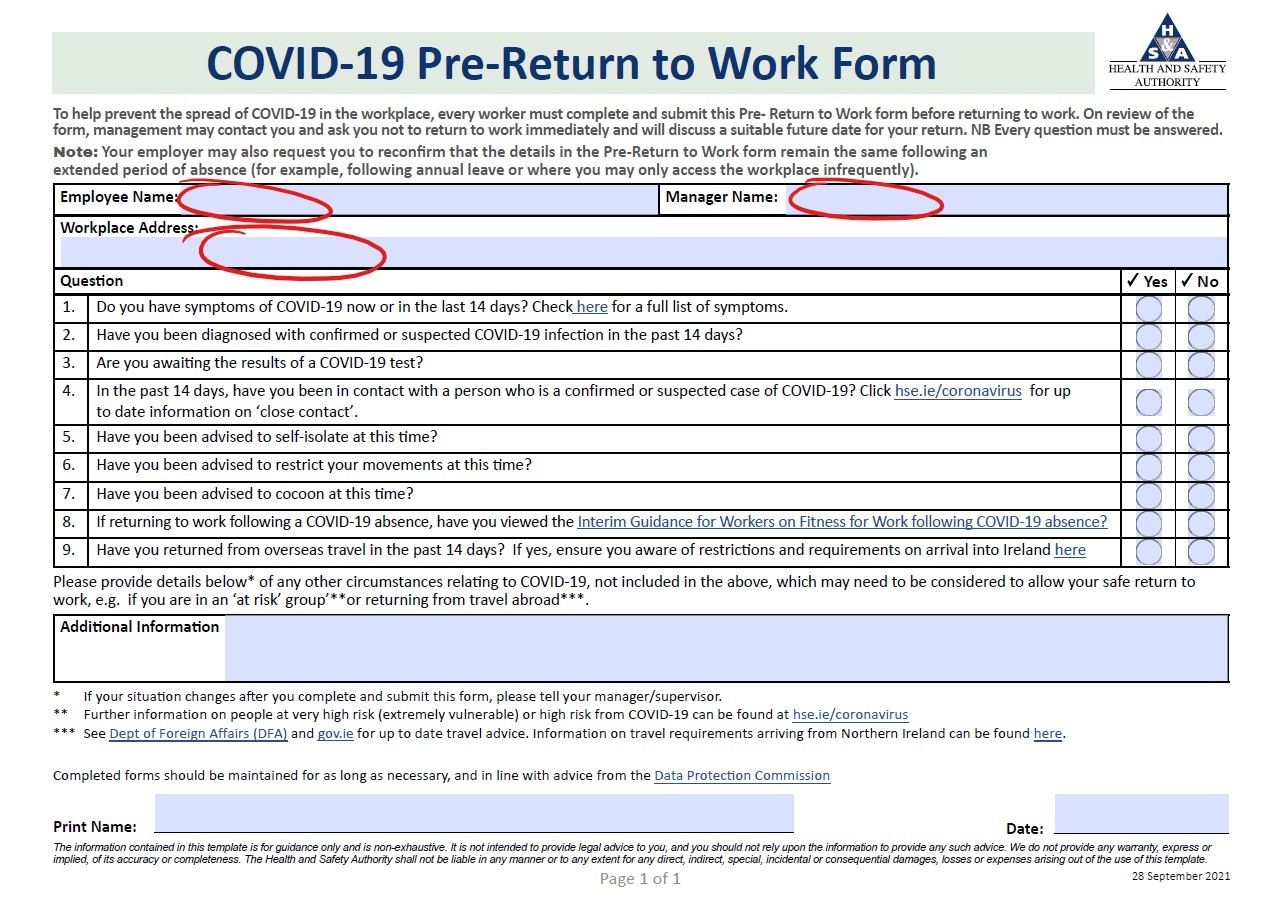
\includegraphics[width=0.7\linewidth]{img/HSAForm}
	\caption{Screenshot of HSA Return to Work Form}
	\label{fig:hsaform}
\end{figure}


Once complete, your batch file should consist of about 12 commands, and the Python code should be about 25 lines of code.

\section*{Extra Credit Section (+20\%)}
An additional 20\% will be awarded, subject to an overall maximum of 100\% for creating a Python program that will also copy the excel files, thus negating the need for the batch file.  In order to qualify for the extra credit portion, you must also submit files in accordance with the standard assignment specification. 

\section*{Testing and Marking}
When marking your work, I will be running the files as submitted.  You should ensure that your batch file and python script(s) have been thoroughly tested before submission.  Code that does not run will score poorly.     


\section*{Submission}
Your submission should comprise of at least two files as shown below:
\begin{enumerate}
	\item Windows Batch File (.bat)
	\item Python Script File (.py)
\end{enumerate}

If you choose to submit the extra-credit section, you must also submit all of the standard submission files.\\
\\
You do not need to submit the excel files as they will be created by me using your batch file and python file where submitted.\\
\\
In any event all parts of your submission are to be uploaded to Teams on or before the submission deadline.

\end{document}